\documentclass[12pt]{article}
\usepackage{geometry}                % See geometry.pdf to learn the layout options. There are lots.
\geometry{letterpaper}                   % ... or a4paper or a5paper or ... 
%\geometry{landscape}                % Activate for for rotated page geometry
%\usepackage[parfill]{parskip}    % Activate to begin paragraphs with an empty line rather than an indent
\usepackage{graphicx}
\graphicspath{{images/}}
\usepackage{amsmath,amssymb,amsfonts,amsthm} 
\usepackage{epstopdf}
\usepackage{epigraph}

% Computer Concrete
%\usepackage{concmath}
%\usepackage[T1]{fontenc}

% Times variants
%
%\usepackage{mathptmx}
%\usepackage[T1]{fontenc}
%
%\usepackage[T1]{fontenc}
%\usepackage{stix}
%
% Needs to typeset using LuaLaTeX:
%\usepackage{unicode-math}
%\setmainfont{XITS}
%\setmathfont{XITS Math}

% garamond
%\usepackage[cmintegrals,cmbraces]{newtxmath}
%\usepackage{ebgaramond-maths}
%\usepackage[T1]{fontenc}

\DeclareGraphicsRule{.tif}{png}{.png}{`convert #1 `dirname #1`/`basename #1 .tif`.png}

\theoremstyle{plain}
\newtheorem{theorem}{Theorem}
\newtheorem{corollary}[theorem]{Corollary}
\newtheorem{lemma}[theorem]{Lemma}
\newtheorem{proposition}[theorem]{Proposition}
\newtheorem{conjecture}[theorem]{Conjecture}
\newtheorem{question}[theorem]{Question}

\theoremstyle{definition}
\newtheorem{definition}[theorem]{Definition}
\newtheorem{example}[theorem]{Example}
\newtheorem*{keywords}{Keywords}
\newtheorem*{sources}{Sources}

\theoremstyle{remark}
\newtheorem{remark}[theorem]{Remark}
\newtheorem{note}[theorem]{Note}
\newtheorem{intuition}[theorem]{Intuition}

\title{Electricity and Magnetism}
\author{Nhan Trong}
\date{\today}                                           % Activate to display a given date or no date

\begin{document}
\maketitle

\epigraph{\textit{Everything should be made as simpa as possiba, but no simpla.}}{Albert Einstein}

\begin{keywords}
Coulomb's Law, electric field, dipole, superposition, infinite uniformly charged plate, parallel plates, charge density, Gaussian surface, Gauss's Law / Flux Theorem, vacuum permittivity / electric constant, Coulomb's Constant, vacuum permeability / magnetic constant.
\end{keywords}

\begin{proposition}[Inverse Cube Law for Dipoles]
The electric field of a dipole varies inversely as the distance cubed.
\end{proposition}

\begin{proposition}
The electric field of an infinite uniformly charged plate is constant and equal to $E = 2 \pi k \sigma = \frac{\sigma}{2 \epsilon}$, where $\sigma$ is the charge density of the plate: the field is the same no matter where you are above the plate. Neat!
\end{proposition}

\begin{proof}
There are two ways to show this, using either Gauss's Law or direct integration. TODO.
\end{proof}

\centerline{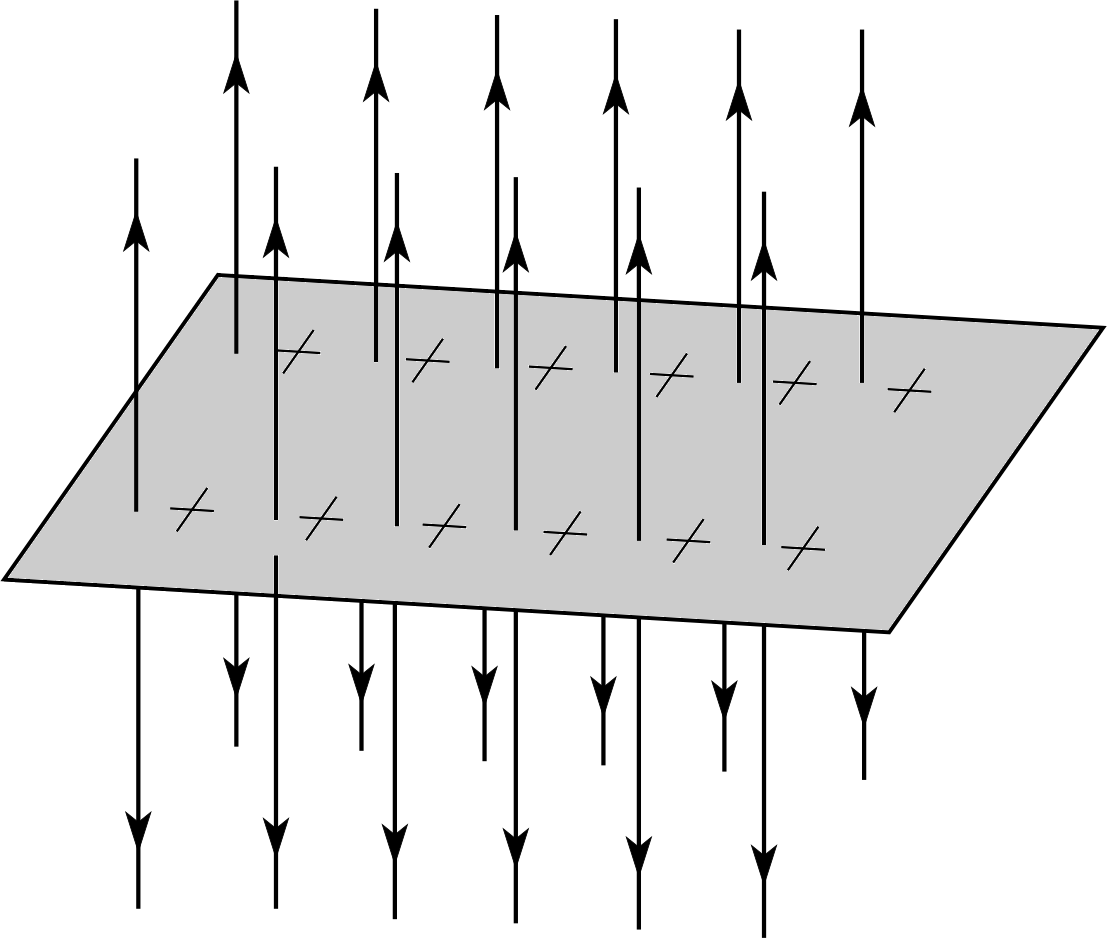
\includegraphics[width=1.0\textwidth]{infiniteplate}}

\begin{corollary}
The electric field of an infinite uniformly charged plate with a hole at the origin is constant along the line above the origin.
\end{corollary}

\begin{question}
What does the rest of the field look like? Do the field lines converge towards the z-axis?
\end{question}

\begin{corollary}
If you had two parallel plates of opposite and equal charge densities, the electric field between the two plates would be twice as big: $E = \pi k \sigma = \frac{\sigma}{\epsilon}$. Beyond those plates the field is zero because the plates cancel each other out.
\end{corollary}

\end{document}
